\section{Evaluation}
\label{sec:evaluation}

Evaluation separates computational reproducibility, deterministic contract behavior, descriptive corpus measurements, and semantic correctness. These categories have different reference standards. A byte-identical replay establishes repeatability of a transformation; a negative control establishes rejection of a specified invalid input; neither establishes the truth of a reconstructed event. Table~\ref{tab:evaluation} reports all ten system experiments with their evidence category and remaining limits. Machine-readable values, source hashes, denominators, environment, and commands accompany the paper in \texttt{audited\_evaluation\_metrics.json}; execution logs are retained separately. No fresh collection or model inference was required for these checks.

\begin{table*}[t]
\centering
\small
\caption{System evaluation matrix. ``Evaluated'' denotes the stated bounded measurement, not independent semantic validation. Historical receipts are distinguished from fresh checks.}
\label{tab:evaluation}
\begin{tabularx}{\textwidth}{@{}p{0.07\textwidth}p{0.19\textwidth}XX@{}}
\toprule
ID & Experiment & Evidence and observed result & Evaluation boundary \\
\midrule
E1 & Reproducibility & Fresh hash checks, exact-graph replay, saved-draw arithmetic, and four 25-draw prefixes agree. & No fresh recrawl; full 9,999-draw generation is a historical replay receipt. \\
E2 & Data collection & Saved historical/expanded counts and missingness independently recomputed. & Integrity and coverage description; platform completeness and relevance recall unknown. \\
E3 & Duplicate detection & Exact sweep: 369 qualifying pairs; 367 retained by legacy candidates; two misses, zero extras. & Conditional finite-corpus candidate recall; no semantic duplicate gold. \\
E4 & Coordination detection & Saved 16-test family: raw $p=.0001$, Holm $p=.0016$; bounded prefixes reproduce. & Conditional exploratory nulls; organic-control specificity and attribution unmeasured. \\
E5 & Evidence retrieval & Captured-corpus retrieval and reference controls exercised by offline tests. & Curated/known inputs; no blind open-web retrieval benchmark. \\
E6 & Claim verification & Abstention, conflict, cutoff, and lineage contract controls pass. & No independent semantic accuracy or entailment score; counterexamples remain material. \\
E7 & Event reconstruction & Typed event organization and synthetic timeline/reference invariants checked. & No autonomous raw-event discovery or independently adjudicated chronology score. \\
E8 & Video/ASR & Historical supplied-reference arithmetic: 185 errors/415 words, 44.58\% micro WER. & Selected clips; independent reference listening provenance not established. \\
E9 & End-to-end workflow & Two clean retrieval-only repeats remain partial/unverified; dangling-event negative control fails. & Two candidates, no accepted support, no generated report; not a blind incident evaluation. \\
E10 & Runtime/resources & Fresh offline suite: 7.84\,s wall, 328,320\,KiB maximum RSS; bounded analytical audit also measured. & Partial local workloads; no current GPU benchmark, API cost, or full-run throughput. \\
\bottomrule
\end{tabularx}
\end{table*}

The fresh full repository suite returned 783 passed tests and 16 passed subtests, with no failures. Pytest reported 7.41\,s; an external resource measurement recorded 7.84\,s wall time and 328,320\,KiB maximum resident memory, exiting successfully. The interpreter was the repository virtual environment's Python 3.13.14 on Linux/x86-64. These counts describe regression coverage, not an accuracy denominator. Six frozen synthetic controls also passed, covering a known microcase, single-root copy fanout, contradictory testimony, correction cutoffs, incomplete evidence, and reused video. Their expected states are known by construction. They are useful release gates without being blind observations of incident truth.

For collection accounting, direct parsing reconciled 23,350 historical publications with 1,408 selected relevant records and 1,384 texts eligible for similarity analysis. The historical 459 missing raw texts and 49 absent view counters belong to all publications; neither is missing among the relevant subset. The remaining 24 relevant texts are shorter than the 80-character eligibility threshold. The expanded snapshot contains 23,386 publications and 1,438 relevant records. These versions are distinct analysis frames. The exact graph and conditional timing tests use the historical frame; a lineage document's assignment of that graph to the expanded frame was rejected against its recorded input hashes. Such checks address denominator integrity without establishing sampling representativeness~\cite{Olteanu2019,VicentePaula2023}.

The duplicate experiment recomputed the entire eligible exact graph using the production five-character shingle definition and 64-bit intersection arithmetic. At Jaccard thresholds .60, .75, and .90, exact cross-channel totals were 369, 288, and 213; legacy retrieval retained 367, 288, and 213. Thus candidate recall at .60 is $367/369=99.45799458\%$, conditional on the 1,384 eligible historical texts. Eighteen same-channel qualifying pairs are excluded by the graph definition. Both missed cross-channel edges exceed 30 minutes, so the observed short-lag counts remain 134 within ten minutes and 198 within thirty minutes, each now divided by 369. Figure~\ref{fig:copy} presents this distinction between candidate retrieval and exact measurement. Shingle sketching supplies a retrieval mechanism, not semantic identity or source dependence~\cite{Broder1997}.

\begin{figure*}[t]
\centering
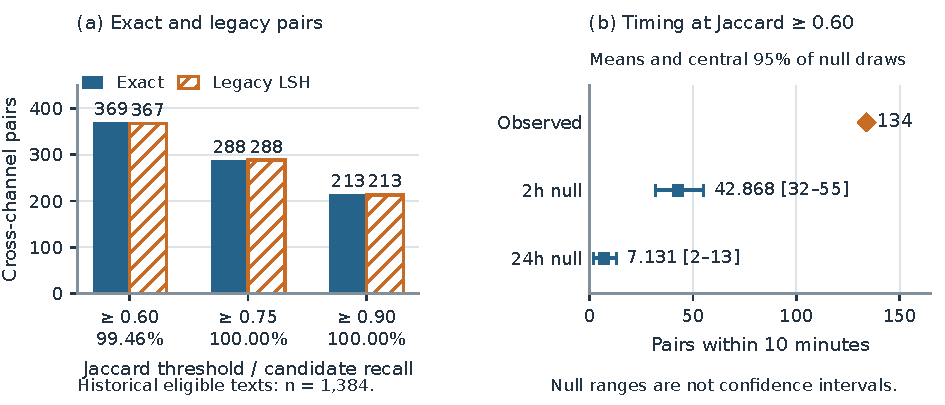
\includegraphics[width=\textwidth]{information_analysis.pdf}
\caption{Finite-corpus similarity retrieval and conditional copy timing. Left: exact versus legacy retained pairs, with recall at each threshold, among 1,384 eligible historical texts. Right: 134 observed pairs at Jaccard $\geq .60$ within ten minutes versus the two saved conditional-null means. Whiskers show the central 95\% of 9,999 randomization draws, not confidence intervals. All timing counts use the fixed 369-edge graph. Sources and hashes are retained in \texttt{data/figure\_data/information\_analysis.json}.}
\label{fig:copy}
\end{figure*}

For coordination, every saved draw was reread and all sixteen summary rows were recomputed, including means, quantiles, upper-inclusive tails, and multiplicity adjustment. With 9,999 draws, all recorded exceedance counts are zero; the plus-one Monte Carlo value is $(0+1)/(9999+1)=.0001$, and Holm adjustment over this declared family gives .0016~\cite{Phipson2010,Holm1979}. A fresh replay reproduced the first 25 draws of each of four models using seed 20261106. This audit did not regenerate all draws. Timing permutations assign one rotated time to each graph node, shared across its edges. Consequently, edges are not treated as independent trials. Departures from these conditional backgrounds do not establish intent, inauthenticity, an organizer, or specificity against matched benign events~\cite{Pacheco2021,Nizzoli2021,Magelinski2022}.

Semantic evaluation remains more limited. The narrative comparison pairs rules with Claude labels on forty selected test posts, rather than independent human adjudication; its agreement statistics cannot validate stance accuracy. Evidence retrieval operates over a captured corpus, and lexical ranking does not establish passage entailment~\cite{RobertsonZaragoza2009BM25}. Curated claim regression checks and synthetic counterexamples are reported as such. Typed event records organize supplied assertions; structural validity does not demonstrate discovery of the underlying physical events. Likewise, the historical ASR error calculation uses supplied reference strings whose independent listening provenance was not established. Its 44.58\% micro WER is descriptive arithmetic for those clips, not a blind corpus-wide recognizer benchmark.

The fresh workflow smoke artifact records two repeat retrieval-only runs with two candidates, an unverified claim, zero accepted support assessments, and no report. A third run deliberately introduces a dangling event evidence reference and correctly fails the evaluation gate. Equal semantic projections across the clean repeats establish bounded repeatability, while their partial status identifies unfinished stages. The combined analytical audit took 4.8317\,s and 1,032,620\,KiB maximum RSS, including corpus loading, exact comparison, saved-draw checking, prefix replay, and graph/bin reconstruction. These resource measurements exclude collection, production ASR, external models, and subsequent auxiliary checks. No current GPU timing or monetary API cost was measured. Independent incident-level evidence, event, and report accuracy therefore remain unmeasured outcomes rather than inferred benefits of a passing software suite.
